\subsection{Polyhedra en het bestaande ontwerp}
\noindent {\em Auteur: Bram Vandendriessche}
\\\\
Het ontwerp van de simulator zorgt ervoor dat de uitbreiding ervan met polyhedra vrij eenvoudig in te voeren is. Door het nieuwe type Polyhedron dat erft van de \textit{WorldObjects}, moesten in \textit{World} zelf slechts enkele extra methodes worden ge\"implementeerd m.b.t. het toevoegen en verwijderen van een Polyhedron aan de bestaande wereld.\\
\noindent
Het ontwerp van het Testbed heeft de grote zwakte dat het erg moeilijk is om individuele elementen en methodes te testen. Dit komt doordat de objecten vaak erg afhankelijk zijn van de wereld waarin ze bestaan. Die wereld is bovendien altijd afhankelijk van de \textit{gl}-component van OpenGL, waardoor het noodzakelijk is een volledige wereld op te zetten voor de test kan worden uitgevoerd. Een oplossing hiervoor zou zijn om de objecten en wereld zo op te splitsen dat presentatie en representatie gesplitst worden, zodat het representatie-gedeelte onafhankelijk kan gebruikt worden. Daarnaast zou dan enkel de wereld weet moeten hebben van haar objecten en niet andersom, zodat objecten onafhankelijk van de wereld kunnen worden getest.\\

\noindent 
De Polyhedron zelf is zo ontworpen dat die bestaat uit verschillende Triangles. De tekenfunctie van de Polyhedron draagt elke Triangle die tot de Polyhedron behoort, op om zichzelf te tekenen. Een Triangle bestaat uit co\"ordinaten voor zijn drie hoekpunten en een kleur voor het buitenste gedeelte van de driehoek. Op basis daarvan worden de binnenste hoekpunten berekend en er wordt een kleur afgeleid uit de gegeven kleur zodat de driehoek voldoet aan de gegeven beperkingen m.b.t. de kleur, zie tabel \ref{table: HSVwaarden}, en de oppervlakte.\\

\noindent

Voor het testen van de Autopilot zijn verschillende figuren ontworpen. Zij vallen onder de \textit{PredefinedPolyhedron}, een subklasse van Polyhedron die ook een positie mee kan krijgen bij creatie. Hierdoor kan de figuur op een gewenste positie worden geplaatst. De standaard Polyhedra krijgen geen positie mee. Hun positie wordt gezet op het massapunt van de polyhedron (de gemiddelde 3D-co\"ordinaat van alle hoekpunten). Op die manier wordt gezorgd dat de positie logisch is t.o.v. de hoekpunten en het niet mogelijk is dat een figuur bijvoorbeeld rond (20,0,0) wordt gedefinieerd, maar wel een positie van (0,0,-40) krijgt toegewezen. De figuren vari\"eren van een eenvoudige met vier hoekpunten tot meer complexe zoals een kubus met een opening in, waarbij de Autopilot zal moeten weten dat het voor de drone niet mogelijk is hierdoor te vliegen.

\begin{figure}
	\centering
	\begin{subfigure}{.5\textwidth}
		\centering
		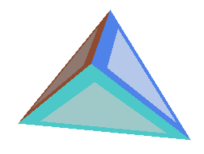
\includegraphics[width=.4\linewidth]{4point.png}
		\caption{Eenvoudige figuur}
		\label{fig:sub1}
	\end{subfigure}%
	\begin{subfigure}{.5\textwidth}
		\centering
		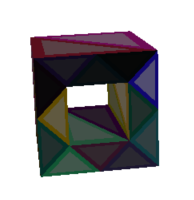
\includegraphics[width=.4\linewidth]{hollowcube.png}
		\caption{Complexere figuur}
		\label{fig:sub2}
	\end{subfigure}
	\caption{Voorgedefinieerde polyhedra.}
	\label{fig:test}
\end{figure}
